% Our first year of experience with PLIDA in ABS DataLab
% (c) 2026 Malcolm Gillies <malcolm.gillies@unsw.edu.au>
% (c) 2026 Kelly Hall <kelly.hall@adelaide.edu.au>
% https://github.com/mbg-unsw/plida-casestudies
%
% This work is licensed under a
% Creative Commons Attribution-NonCommercial-ShareAlike 4.0
% International Licence
\documentclass[aspectratio=169,12pt]{beamer} % XXXX fix AR here
\usepackage{pgfpages}
\usepackage{fancyvrb}
\usepackage{pgfplots}
%\usepackage[latin1]{inputenc}
%\usepackage[T1]{fontenc}
%\usepackage{textcomp}
%\usefonttheme{serif} % need this with Charter font
\usetheme{auriga}  % using default now
\usecolortheme{auriga}  % using default now
%\usepackage[libertine]{libertine} % not using osf (old-style figures)
%\usepackage[scale=0.9]{tgheros} % scale to match libertine
%\usepackage[varqu,varl]{inconsolata}
%\usepackage[libertine]{newtxmath}
\usepackage{graphicx}
\usepackage{tikz}
\usetikzlibrary{shadows}
\usepackage{tikzpagenodes}
\usepackage{natbib}
\usepackage{gitinfo2}

\pgfplotsset{compat=1.17}
\hypersetup{pdfencoding=auto}

\renewcommand{\gitMark}{\color{lightgray}\texttt{\tiny\gitBranch\,@\,\gitAbbrevHash\,\gitAuthorDate}}

%\renewcommand{\bibsection}{} % suppress "References" section

%\setbeamertemplate{navigation symbols}{} % remove navigation symbols
%\setbeamercolor*{item}{fg=darkred}

\title{Hands on with PLIDA in ABS DataLab}
\author{Malcolm Gillies <malcolm.gillies@unsw.edu.au>\\
Kelly Hall <kelly.hall@adelaide.edu.au>}
\institute{16 June 2026}
\usebackgroundtemplate{%

\includegraphics[width=\paperwidth]{ref/micre-blank.PNG}
\begin{tikzpicture}[remember picture,overlay]
    \node[anchor=south east,scale=1,rotate=90] at ([shift={(0cm,0cm)}]current page marginpar area.north east) {\gitMark};
\end{tikzpicture}%
}


\newif\ifsidebartheme
\sidebarthemefalse

\newdimen\contentheight
\newdimen\contentwidth
\newdimen\contentleft
\newdimen\contentbottom
\makeatletter
\newcommand*{\calculatespace}{%
    \contentheight=\paperheight%
    \ifx\beamer@frametitle\@empty%
        \setbox\@tempboxa=\box\voidb@x%
      \else%
        \setbox\@tempboxa=\vbox{%
          \vbox{}%
          {\parskip0pt\usebeamertemplate***{frametitle}}%
        }%
        \ifsidebartheme%
          \advance\contentheight by-1em%
        \fi%
      \fi%
    \advance\contentheight by-\ht\@tempboxa%
    \advance\contentheight by-\dp\@tempboxa%
    \advance\contentheight by-\beamer@frametopskip%
    \ifbeamer@plainframe%
    \contentbottom=0pt%
    \else%
    \advance\contentheight by-\headheight%
    \advance\contentheight by\headdp%
    \advance\contentheight by-\footheight%
    \advance\contentheight by4pt%
    \contentbottom=\footheight%
    \advance\contentbottom by-4pt%
    \fi%
    \contentwidth=\paperwidth%
    \ifbeamer@plainframe%
    \contentleft=0pt%
    \else%
    \advance\contentwidth by-\beamer@rightsidebar%
    \advance\contentwidth by-\beamer@leftsidebar\relax%
    \contentleft=\beamer@leftsidebar%
    \fi%
}
\makeatother

\begin{document}

\setbeamercolor{page number in head/foot}{fg=white}

{
\usebackgroundtemplate{
\includegraphics[width=\paperwidth]{ref/micre.PNG}}
\setbeamercolor{title page}{fg=white}
  \begin{frame}[plain]
    \titlepage
  \end{frame}
}

\begin{frame}{}
\calculatespace%
\begin{columns}
\begin{column}{0.25\contentwidth}
\begin{tikzpicture}
  \node[drop shadow={shadow xshift=.8ex,shadow yshift=-.8ex},fill=white,draw] at (0,0) {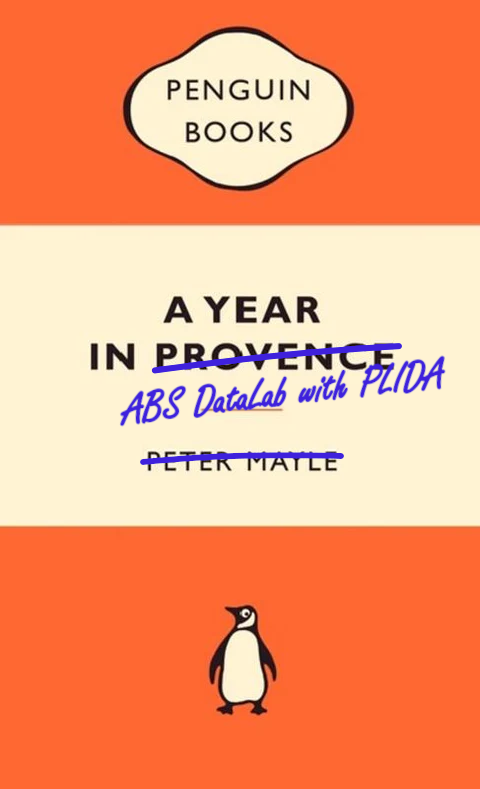
\includegraphics[width=\textwidth]{ref/a-year-in-plida-20260513.png}};
\end{tikzpicture}
\end{column}
\begin{column}{0.50\contentwidth}
ABS PLIDA provides access to a lot of amazing linked Commonwealth data
using the DataLab Trusted Research Environment (TRE). But what's it like
to work with?
\end{column}
\end{columns}
\end{frame}

\begin{frame}{Good stuff\dots}
\begin{itemize}
	\item Fresh data
	\item Straightforward process for publication
	\item Modern environment, regular software updates, good VM spec
	\item Extensive docs and transparent processes
	\item Responsive staff
	\item Harmonised data in core demographics
\end{itemize}
\end{frame}

\begin{frame}{Datasets we've used in PLIDA}
\begin{itemize}
	\item Pharmaceutical Benefits Scheme (PBS)
	\item Census 2021
	\item Core demographics
	\item Core location
	\item PLIDA spine
\end{itemize}
\end{frame}

\begin{frame}{Research topics so far\dots}
\begin{itemize}
	\item 60-day prescribing on the PBS
	\item ADHD--CVD medicine drug--drug interaction
	\item ADHD medicine geographic variation
\end{itemize}
\end{frame}

{
\usebackgroundtemplate{
\begin{tikzpicture}[remember picture,overlay]
    \fill[black]([shift={(0cm,0cm)}]current page.north west)
	rectangle
   ([shift={(0cm,0cm)}]current page.south east);
\end{tikzpicture}%
}
\setbeamercolor{background canvas}{bg=black}
  \begin{frame}[plain]
	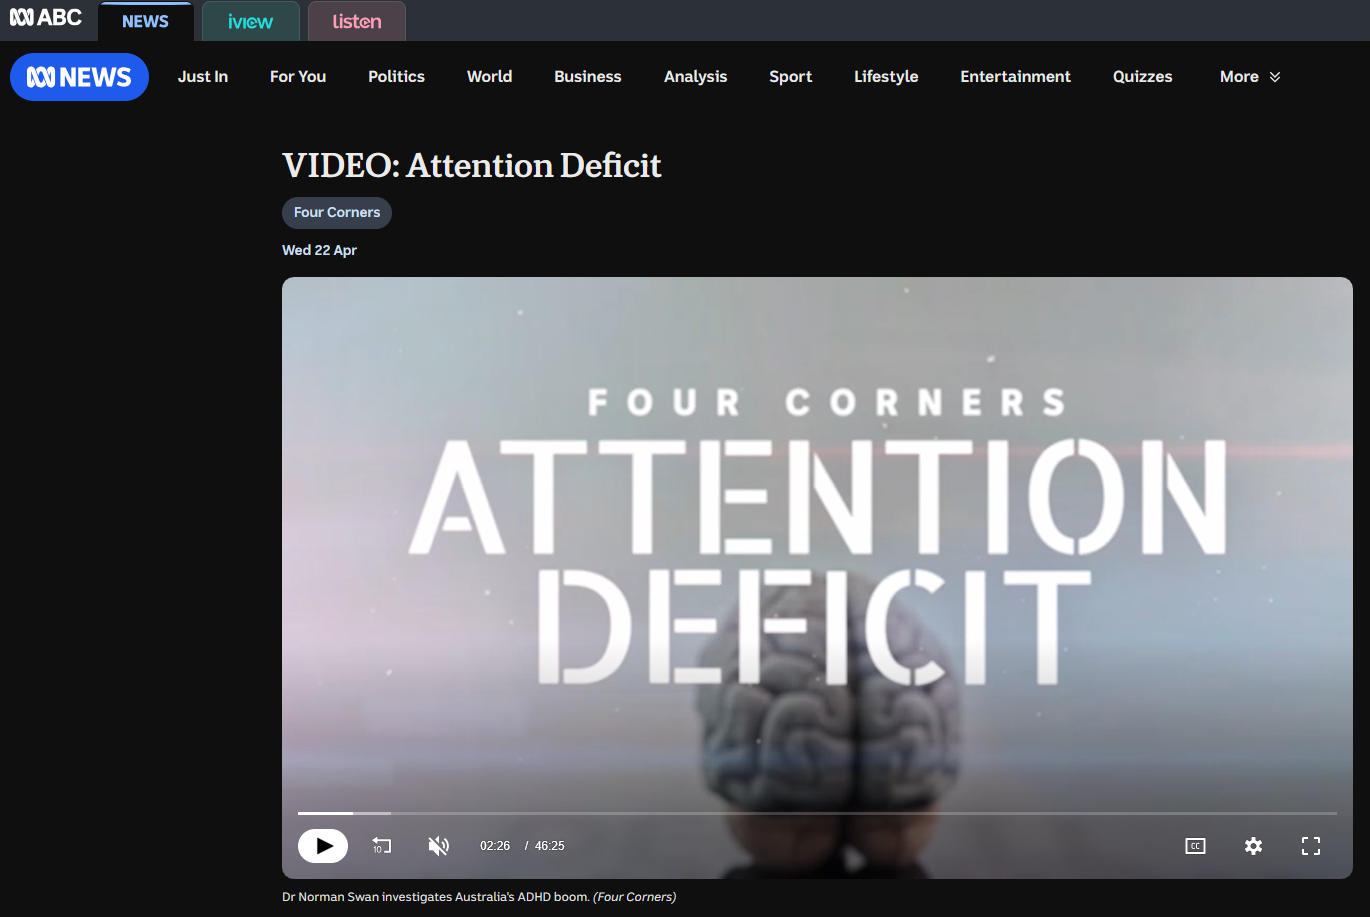
\includegraphics[height=\paperheight]{ref/4corners-grab-20260513.png}
  \end{frame}
}

\begin{frame}{}
\calculatespace%
\begin{columns}
\begin{column}{0.40\contentwidth}
  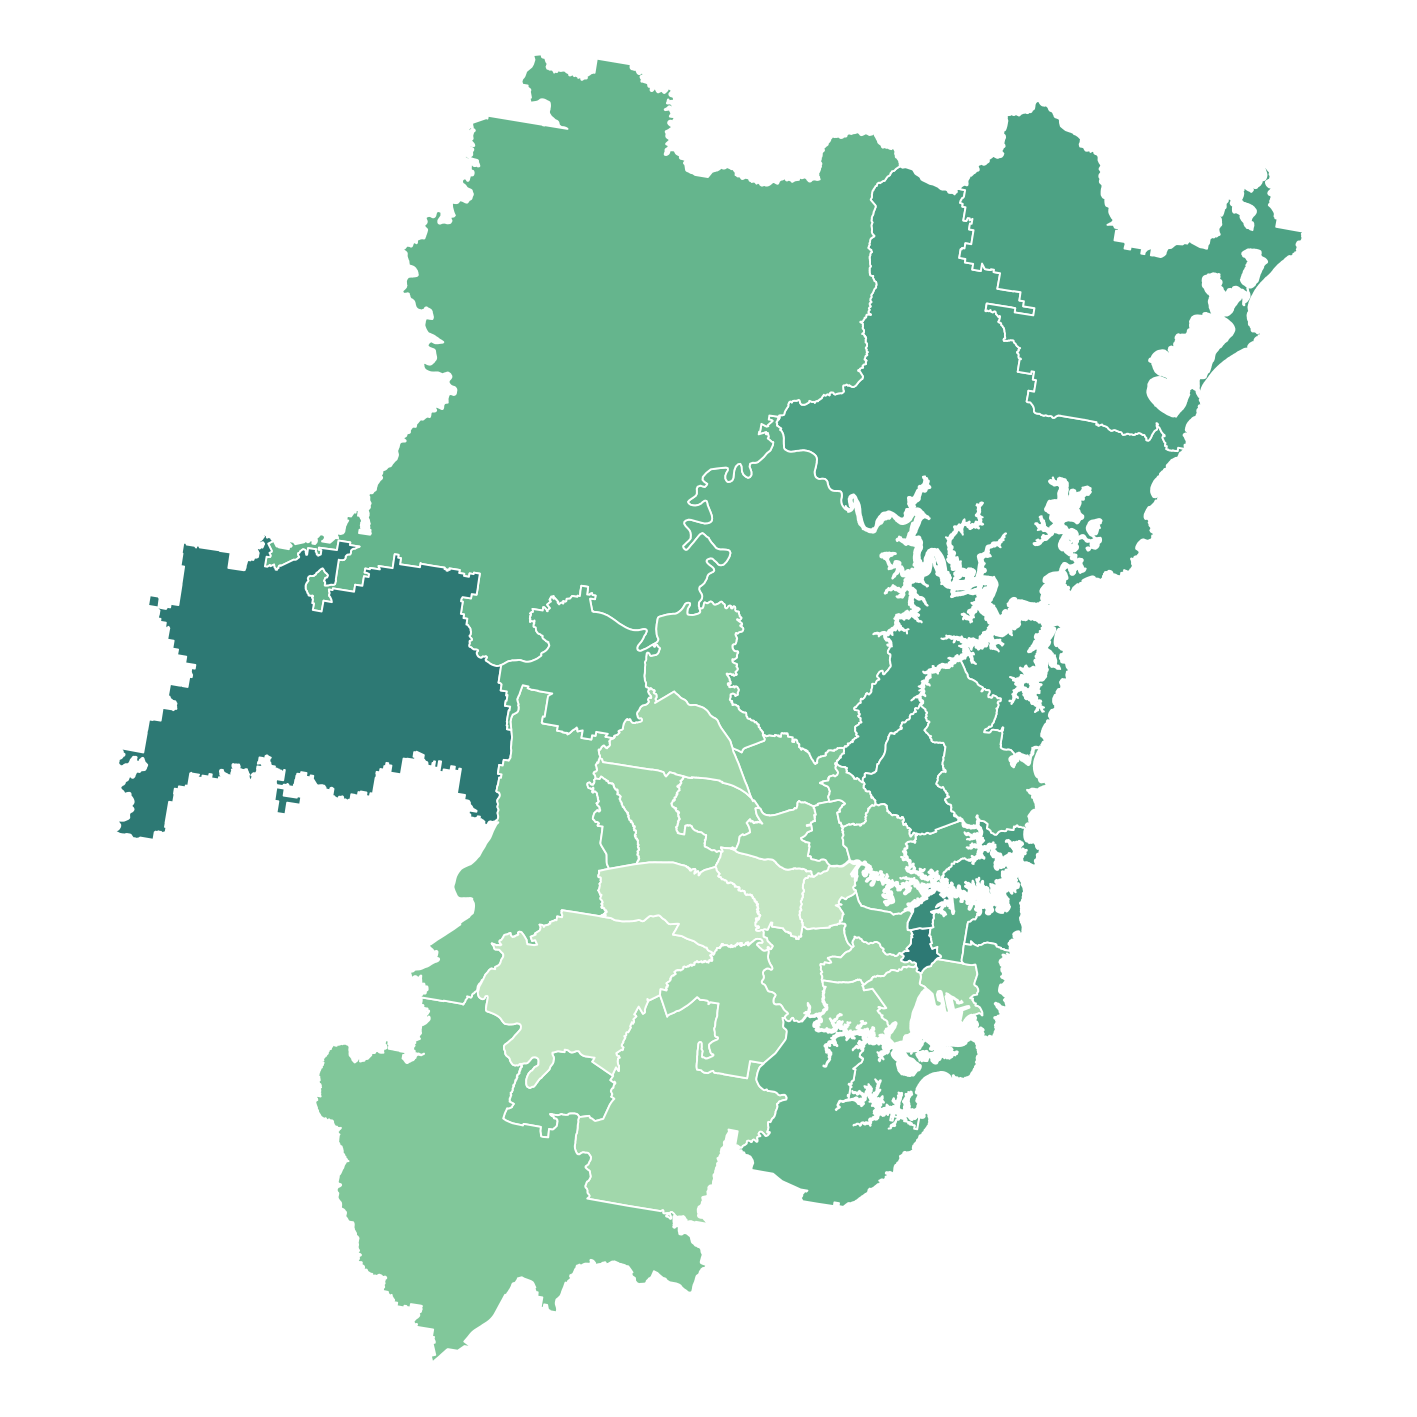
\includegraphics[width=\textwidth]{ref/map_prev_syd.png}
\end{column}
\begin{column}{0.45\contentwidth}
	\begin{itemize}
	    \item Annual prevalence of ADHD medicine dispensing for 2023--24
	    \item Age standardised population rate per SA3
	    \item Exported from DataLab in tabular form
	    \item Visualisation using \texttt{\{tmap\}}
	\end{itemize}
\end{column}
\end{columns}
\end{frame}

\begin{frame}{Some things I learned (Malcolm)}
\begin{itemize}
	\item Bigger data, slower analyses (new tools help)
	\item Nightly automatic shutdown: don't forget
	\item Quarterly updates: how to manage?
	\item SYNTHETIC\_AEUID ain't SYNTHETIC\_AEUID
	\item Docs are great but sometimes outdated
\end{itemize}
\end{frame}

\begin{frame}{Tips for new starters (Malcolm)}
\begin{itemize}
	\item Request a 1TB X: drive (it's free)
	\item Get to know the size of the data
	\item Create sample data for testing your code
	\item Do reproducible analyses you can show ABS
	\item Explore Census data quirks
\end{itemize}
\end{frame}

\begin{frame}{Advice from a PLIDA survivor (Kelly)}
\begin{itemize}
	\item Give yourself time
	\item Start with the right set up
	\item Before you dive in, learn how the datasets fit together
	\item Read the documentation
	\item Phone a friend
\end{itemize}
\end{frame}

% \begin{frame}{References}
% %        \bibliographystyle{apalike}
% %        \bibliographystyle{abbrv}
%         \tiny\bibliography{plida-casestudies.bib}
%         \bibliographystyle{abbrvnat}
% \end{frame}

\end{document}
